\chapter{Background \& Related Work}
\label{ch:background}
In this chapter,
we will give an introduction to the different fields touched by our research.
Related work is mentioned primarily in section~\ref{ch:background:se:graphDatabaseBenchmarks} as it covers the different benchmarks and their findings.

\section{Graphs}
\label{ch:background:se:graphs}
A graph as the literature tells us~\cite[89]{Worsch2011} is a tuple $ G = (V, E) $ where $ E \subseteq V \times V $.
Elements of $ V $ are called vertices and elements of $ E $ are called edges.
The set of vertices has to be non-empty,
but the edge set can be.
In this thesis we are focusing on directed graphs only,
although some graph databases are capable of handling undirected graphs too.
Also there would be no benefit in using undirected edges since our model also uses directed edges.
In general graphs can have labels or weights on their edges as stated in~\cite[99]{Worsch2011}.
For our purposes we will use labels on the vertices and edges to ease the understanding of our data structure.
In section~\ref{ch:background:se:graphDatabases} we will give reasons why having labels on the graph components is useful.

Figure~\ref{fig:simpleGraph} shows an example of a directed graph with labels on its vertices.
An equivalent representation of that graph would be
\begin{equation}
  \begin{aligned}
    V &= \{1, 2, 3\} \\
    E &= \{(1, 2), (1, 3), (2, 1), (3, 2)\}.
  \end{aligned}
\end{equation}

\begin{figure}[h]
  \centering
  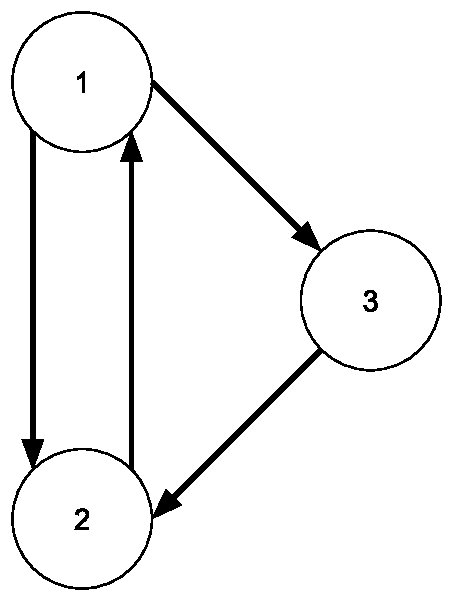
\includegraphics[width=\textwidth/4]{images/simpleGraph}
  \caption{A directed graph with three labelled vertices and four edges.}
  \label{fig:simpleGraph}
\end{figure}

\section{Industrial Data}
\label{ch:background:se:industrialData}
Under the term "industrial data" we understand data which is produced by machines during the production.
That could be the current settings of the machine,
temperatures or tolerances measured during processing or what product is currently worked on.
In chapter~\ref{ch:analysis:se:data} the possible structure of this data is analysed.

As there is no publicly available information about how industrial data should look like we will use the example given by our partners at SICK AG~\cite{SICK} as an inspiration for our test data.

Listing~\ref{lst:exampleData} shows the graph excerpt of our given example.

\begin{lstlisting}[language={XML},label={lst:exampleData},caption={An excerpt showing the observation of components.},captionpos=b]
"@graph": [
  {
    "@id": "http://localhost:3000/observations/185",
    "@type": "ssn:Observation",
    "featureOfInterest": "aoi:Feature",
    "observationSamplingTime": "2016-05-18T12:55:27.954Z",
    "observedProperty": [
      "aoi:twisting",
      "aoi:y-shift",
      "aoi:x-shift"
    ],
    "observationResult": "http://localhost:3000/observations/185/sensor-output",
    "observationResultTime": "2016-05-18T12:55:27.954Z",
    "observedBy": "http://localhost:3001/AOI_SMD407",
    "dataClass": "Testdata"
  },
  {
    "@id": "http://localhost:3000/observations/185/sensor-output",
    "@type": "ssn:SensorOutput",
    "isProducedBy": "http://localhost:3001/equipment/AOI_SMD407",
    "hasValue": "http://localhost:3000/observations/185/result"
  },
  {
    "@id": "http://localhost:3000/observations/185/result",
    "@type": "ssn:ObservationValue, shopfloor:Panel",
    "orderNo":"http://localhost:3000/order#0",
    "partNr": "http://localhost:3000/part#2060817",
    "hasPart": "http://localhost:3000/observations/185/board#3827581",
    "startTime": "2016-05-18T12:55:27.954Z",
    "endTime": "2016-05-18T12:56:27.954Z"
  },
  {
    "@id": "http://localhost:3000/observations/185/board#3827581",
    "@type": "shopfloor:Board",
    "hasPart": ["http://localhost:3000/observations/185/component#C1-1","http://localhost:3000/observations/185/component#C2-1"],
    "boardUID":"3827581",
    "isBadBoard": false
  },
  {
    "@id": "http://localhost:3000/observations/185/component#C1-1",
    "@type": "shopfloor:Component",
    "componentType": "C0603",
    "position":0,
    "testFeature":[
      {
        "@id": "http://localhost:3000/observations/185/component#C0603-MENI-901-TWISTING",
        "feature": "aoi:twisting1",
        "analysisMode": [
          {"@id": "http://localhost:3000/observations/185/AnalysisMode#C0603-MENI-901-TWISTING",
            "windowNumber": "901",
            "featureFlag": "0",
            "mode":"MENI"
          }
        ],
        "hasValue": {
          "@type": "xsd:integer",
          "@value": "10"
        }

      },
      {
        "@id": "http://localhost:3000/observations/185/component#C0603-MENI-901-Y-Shift",
        "feature": "aoi:y-shift1",
        "analysisMode": [
          {"@id": "http://localhost:3000/observations/185/AnalysisMode#C0603-MENI-901-Y-Shift",
            "windowNumber": "901",
            "featureFlag": "0",
            "mode":"MENI"
          }
        ],
        "hasValue": {
          "@type": "xsd:integer",
          "@value": "-17"
        }
      },
      {
        "@id": "http://localhost:3000/observations/185/component#C0603-MENI-901-X-Shift",
        "feature": "aoi:x-shift1",
        "analysisMode": [
          {"@id": "http://localhost:3000/observations/185/AnalysisMode#C0603-MENI-901-X-Shift",
            "windowNumber": "901",
            "featureFlag": "0",
            "mode":"MENI"
          }
        ],
        "hasValue": {
          "@type": "xsd:integer",
          "@value": "20"
        }
      }
    ]
  },
  {
    "@id": "http://localhost:3000/observations/185/component#C2-1",
    "@type": "aoi:Component",
    "componentType": "C0603",
    "position":0,
    "testFeature":[
      {
        "@id": "http://localhost:3000/observations/185/component#C0603-MENI-901-TWISTING",
        "feature": "aoi:twisting1",
        "analysisMode": [
          {"@id": "http://localhost:3000/observations/185/AnalysisMode#C0603-MENI-901-TWISTING",
            "windowNumber": "901",
            "featureFlag": "0",
            "mode":"MENI"
          }
        ],
        "hasValue": {
          "@type": "xsd:integer",
          "@value": "12"
        }
      },
      {
        "@id": "http://localhost:3000/observations/185/component#C0603-MENI-901-Y-Shift",
        "feature": "aoi:y-shift1",
        "analysisMode": [
          {"@id": "http://localhost:3000/observations/185/AnalysisMode#C0603-MENI-901-Y-Shift",
            "windowNumber": "901",
            "featureFlag": "0",
            "mode":"MENI"
          }
        ],
        "hasValue": {
          "@type": "xsd:integer",
          "@value": "14"
        }
      },
      {
        "@id": "http://localhost:3000/observations/185/component#C0603-MENI-901-X-Shift",
        "feature": "aoi:x-shift1",
        "analysisMode": [
          {"@id": "http://localhost:3000/observations/185/AnalysisMode#C0603-MENI-901-X-Shift",
            "windowNumber": "901",
            "featureFlag": "0",
            "mode":"MENI"
          }
        ],
        "hasValue": {
          "@type": "xsd:integer",
          "@value": "11"
        }
      }
    ]
  }
]
\end{lstlisting}

In figure~\ref{fig:exampleData} the provided example is visualised partially.
It shows the observation of a product.

\begin{figure}
  \centering
  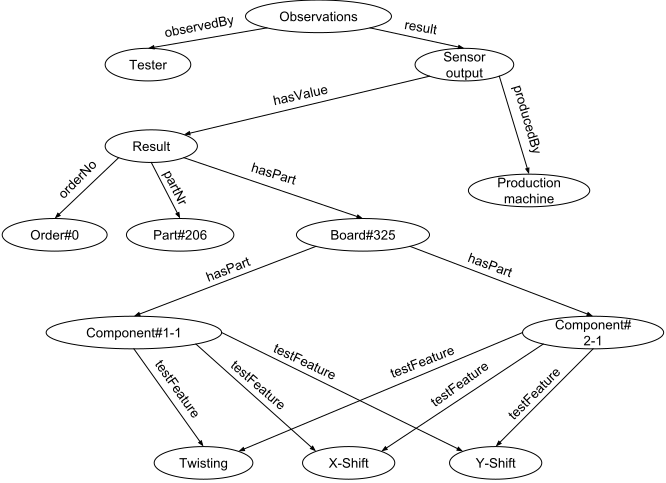
\includegraphics[width=\textwidth]{images/design/exampleGraph}
  \caption{An example graph representing the observation of a board created after the example shown in listing~\ref{lst:exampleData}.}
  \label{fig:exampleData}
\end{figure}

\section{Graph Databases}
\label{ch:background:se:graphDatabases}
There is a variety of database types available and the main categories are SQL and NoSQL databases.
A short description of SQL databases would be
\blockquote[\cite{ChuaHock-Chuan}]{A relational database organizes data in tables (or relations).
A table is made up of rows and columns.
A row is also called a record (or tuple).
A column is also called a field (or attribute).
A database table is similar to a spreadsheet.}

NoSQL databases,
on the other hand,
are able to store any kind of data in any record.
They don't rely on a specified schema and they are able to scale horizontally at the expense of consistency.~\cite{Yegulalp2017}

Graph databases are a type of NoSQL databases.
They use graph theory to store their data as described in section~\ref{ch:background:se:graphs}.
Every vertex and every edge has an unique identifier (id) in the database.
Properties can be assigned to edges and nodes as key/value pairs.
Additionally edges store a reference to the start and end node they are attached to.~\cite{Rouse2016}

The labels mentioned at the end of section~\ref{ch:background:se:graphs} can be seen as the properties assigned to a vertex or edge.
To map a production line in which the elements like machines and products have their own real-world ids,
a property can be used to store these ids as key/value pairs.
Later a particular machine,
for example,
can be looked up by its id.
That is crucial to find the data stored in the database.

In the following subsections~\ref{ch:background:se:rdfTriplestores} through~\ref{ch:background:se:graphStores} we will discuss the different types of graph databases and give examples of real databases which operate by that type.
All databases used in this thesis support the ACID\footnote{short for atomicity, consistency, isolation, durability. It should guarantee data validity.} principle and transactions.

\subsection{RDF/Triplestores}
\label{ch:background:se:rdfTriplestores}
First on our list are RDF stores also known as triple stores.

RDF (Resource Description Framework) is a model for data interchange on the web.
It is able to merge data even with different schemas, it also supports the evolution of a schema over time.
The linking structure of the web is extended by RDF by it using URIs\footnote{abbreviation of Universal Resource Identifier, used to identify abstract of physical resources.~\url{https://tools.ietf.org/html/rfc3986}} to name relationships and resources connected by those relationships.~\cite[4]{Ontotext2014}

\blockquote[\cite{W3C2014}]{This linking structure forms a directed, labelled graph, where the edges represent the named link between two resources, represented by the graph nodes.
This graph view is the easiest possible mental model for RDF and is often used in easy-to-understand visual explanations.}

Triplestores store semantic facts as subject - predicate - object triples,
also referred to as statements using RDF.
These statements form a network of data,
which can also be seen as a graph.~\cite[4]{Ontotext2014}

\subsubsection{Apache Jena TDB}
\label{ch:background:se:apacheJena}
\blockquote[\cite{Apache2015}]{Apache Jena (or Jena in short) is a free and open source Java framework for building semantic web and Linked Data applications.
The framework is composed of different APIs interacting together to process RDF data.}

Jena stores its information in statements as triples of subject, predicate and object.
This structure can be seen as a graph, with the subject and the object being vertices and the predicate as an edge between them.

Jena TDBs dataset consists of the node table, triple and quad indices and the prefix table.
The node table contains the representation of RDF terms and provides a mapping from Node to NodeId and the other way around.
Triple and quad indices are indices for the default graph and named graphs respectively.
The triple indices contain three indices for the three parts of a statement.
Each index has all information about the triple,
there is no secondary index.
Prefixes table are mainly used in presentation and serialisation of the triples in RDF/XML or Turtle.~\cite{ApacheTDB}

\subsection{Document Stores}
As the name suggests the data model of document stores consist of documents which can have fields without depending on a defined schema.~\cite{OrientDB}
It aggregates data in those documents and transforms them internally into a searchable form.~\cite{Techopedia2017}

\subsubsection{OrientDB}
OrientDB is a mix of a document store and a graph store,
as stated in their manual \textquote[\cite{OrientDB}]{OrientDB is a document-graph database, meaning it has full native graph capabilities coupled with features normally only found in document databases.}
It's designed as a robust, highly scalable database with a wide possible set of use cases.~\cite{OrientDB}
OrientDB doesn't require a fixed schema and therefore supports schema-less and schema-mixed models.
It uses an indexing algorithm called MVRB-Tree,
which derived from the Red-Black Tree and the B+ Tree and therefore it supports fast insertions as well as fast lookups.~\cite{Abubakar2014}

\subsection{Graph Stores}
\label{ch:background:se:graphStores}
Graph stores organise their data as graphs.
References with foreign keys known from relational databases are mapped as relationships in graph databases.
Each node in the database model contains a list of relationship-records to represent their connection to other nodes.~\cite{NeoTechnologyInc.2016}

\subsubsection{Neo4j}
Neo4j is a native graph database and was built as such from the ground up.
It organises its data in a graph structure and has nodes, relationships and attributes as directly accessible data structures.
It can assign attributes to both nodes and edges.
Neo4j is transactional and fulfils the ACID properties.~\cite{Neo4jInc.2006}

\subsubsection{Sparksee}
The user manual describes Sparksee as follows, \textquote[\cite{SparsityTechnologies}]{Sparksee is an embedded graph database management system tightly integrated with the application at code level.}
Sparksee is implemented in C++ and provides a Java API.

Sparksee encodes its nodes and edges as collections of objects, which all have a unique identifier.
It implements two types of structures, bitmaps and maps.
Adjacency matrices are converted into multiple small indices,
which improves the out-of-core workloads.
Sparksee uses also efficient I/O and cache policies.
The bitmaps in which the adjacency list of each node is stored are typically sparse in graphs and they are therefore compressed to save space.
Attributes,
which are stored in a B-Tree,
are supported for both nodes and edges.
Two maps are used.
One which maps the object id to the attribute and the other one mapping the attribute value to the object ids that have that value.~\cite{TaoShen}

\section{Graph Database Benchmarks}
\label{ch:background:se:graphDatabaseBenchmarks}
As the need to compare similar programs exists benchmarks are needed to hand results over certain aspects to aid decision making.
In the field of graph databases that is no different.
There exist multiple benchmarks for graph databases and some are outlined shortly in the following subsections~\ref{ch:background:se:ldbcGraphalytics}~to~\ref{ch:background:se:XGDBench}.
In section~\ref{ch:analysis:se:benchmark},
we choose a benchmark for our work.

\subsection{LDBC: Graphalytics}
\label{ch:background:se:ldbcGraphalytics}
Benchmark specifications, practices and results for graph data management systems are established by an industry council called "The Linked Data Benchmark Council".
The Graphalytics benchmark facilitates a choke-point design to evaluate the crucial technological challenges present in system design.
One example would be the "large graph memory footprint" as mentioned in~\cite[2]{Capota2015}.

Graphalytics uses Datagen to create social network graphs,
which are easy to understand for their users.~\cite[3]{Capota2015}

The workloads implemented in Graphalytics represent common graph algorithms such as "breadth-first search",
"weakly connected components" or "single-source shortest paths" to name just a few.~\cite[7]{Iosup}

Figure~\ref{fig:graphalyticsArchitecture} shows the architecture of the Graphalytics benchmarking software.
The user can configure the available benchmarks inside Graphalytics with a benchmark configuration (2).
Parameters for the algorithm included in (1) can be specified and the system under test (4) can be set up.
The system on which the benchmark runs has to be provided by the user.
The harness service (5) coordinates the benchmark configuration and the benchmarking process.
The dataset for the benchmark has to be provided by the user or can be generated by using the available workload generators.~\cite[11]{Iosup}

\begin{figure}[h!]
  \centering
  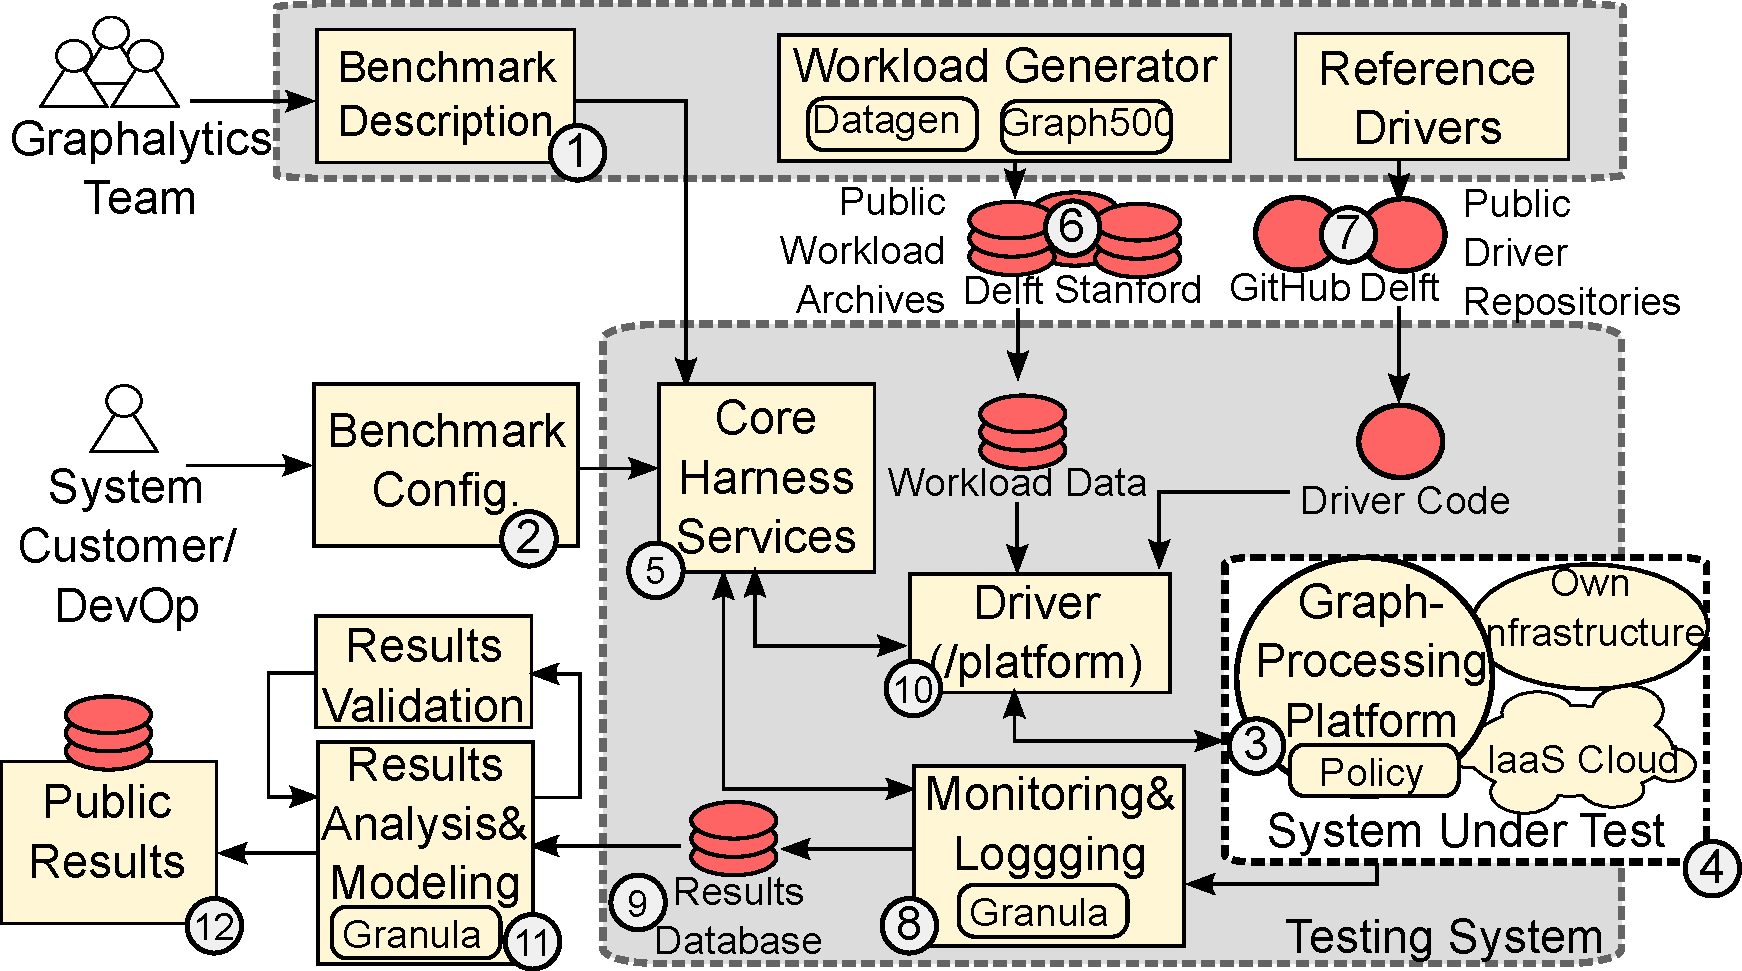
\includegraphics[width=.75\textwidth]{images/benchmarks/GraphalyticsArchitecture}
  \caption{The architecture of the Graphalytics benchmark.~\cite[11]{Iosup}}
  \label{fig:graphalyticsArchitecture}
\end{figure}

\subsection{YCSB}
\label{ch:background:se:ycsb}
The Yahoo! Cloud Serving Benchmark (YCSB) wasn't designed specifically for graph databases,
but rather for key-value and cloud stores.
The client is extensible so that new workloads,
databases and generators can be integrated.~\cite{Yahoo!2010}

The core workload is designed to use simple CRUD\footnote{CRUD stands for the basic operations on persistent storage, these are Create, Read, Update, Delete.} operations on any database with no special structure of the generated data.

The architecture of YCSB can be seen in figure~\ref{fig:ycsbArchitecture}.
The client contains a \texttt{Workload executor} that uses \texttt{Generator}s to create a dataset and executes operations on the database.
Each \texttt{Client thread} calls the \texttt{Workload executor} to perform an operation on the database.
Workload files can be specified to set the amount of data and the mix of operations to use for that workload.
To tell YCSB which database should be used command-line parameters are passed to the client.
The benchmark supports two phases,
a load phase to fill the database with initial data and a transaction phase to execute operations on the database.

\begin{figure}[h!]
  \centering
  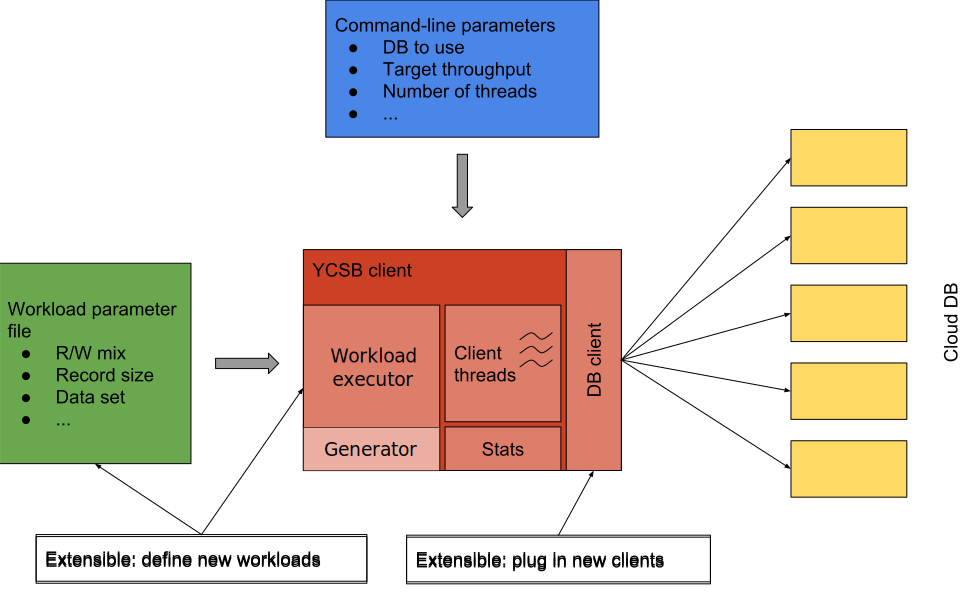
\includegraphics[width=\textwidth]{images/benchmarks/ycsbArchitecture}
  \caption{The architecture of YCSB. Recreated and modified from~\cite[25]{Abubakar2014}.}
  \label{fig:ycsbArchitecture}
\end{figure}

\subsection{XGDBench}
\label{ch:background:se:XGDBench}
Is a graph database benchmark for cloud computing systems.
It is designed to work in the cloud and in future exascale clouds.
XGDBench is an extension of YCSB for graph databases.
This benchmark is written in X10,
a \textquote[\cite{Dayarathna2012}]{programming language that is aimed
for providing a robust programming model that can withstand the architectural challenges posed by multi-core systems,
hardware accelerators, clusters, and supercomputers}.

XGDBench also focuses on social networks for their data structure.
The data is generated by a procedure called "Multiplicative Attribute Graph" (MAG),
see~\cite{Kim2012} for more information.

It specifically targets read,
update and graph traversal operations for its performance aspects.~\cite[366]{Dayarathna2012}

In figure~\ref{fig:XGDBenchArchitecture} the architecture of the XGDBench benchmark is illustrated.
The general workflow is similar to the one from YCSB,
because this benchmark is based on YCSB.
The workload is executed in two phases,
the load phase fills the database with data and the transaction phase executes operations on the database.

\begin{figure}[h!]
  \centering
  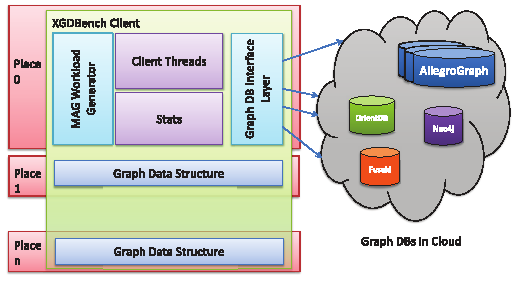
\includegraphics[width=.75\textwidth]{images/benchmarks/XGDBenchArchitecture}
  \caption{The architecture of the XGDBench benchmark.~\cite[367]{Dayarathna2012}}
  \label{fig:XGDBenchArchitecture}
\end{figure}

\section{Related Work}
A number of studies have been conducted to test the performance of NoSQL databases,
which we will discuss in this section.
\todo{Revisit}

\subsection{Evaluation of NoSQL Systems using YCSB}
Abubakar et al. haven't focused their research on graph databases,
but the used OrientDBs document API among others.
They compared the following NoSQL databases MongoDB, ElasticSearch, OrientDB and Redis.
Three different workloads were used in their study,
each concentrating on one operation,
which were inserts, reads and updates.
The dataset size was varied between 1.000 and 100.000 records with a record size of 1KB.
Their insert workload showed that OrientDB was the slowest among the examined database across all dataset sizes whereas Redis was the fastest in this category.
The read workload had no consistent order for the databases,
for every dataset size another database was the best with ElasticSearch as the fastest for the largest dataset.~\cite{Abubakar2014}

\subsection{HPC Scalable Graph Analysis Benchmark}
Dominguez-Sal et al. implemented the HPC Scalable Graph Analysis Benchmark and tested the performance of four different graph databases.
In their research they examined Neo4j, Jena (RDF), HypergraphDB and DEX (Sparksee) with four different workloads covering insert performance, looking up a set of edges, building subgraphs by utilising breadth first search and finally the traversal performance.
They used a dataset generated by the R-MAT algorithm with the parameters $ a = 0.55, b = 0.1, c = 0.1 $ and $ d = 0.25 $.
The final dataset had a composition of nodes to edges of $ N = 2^(scale) $ and $ E = 8 \times N $ with weights on the edges uniformly distributed with a maximum value of $ 2^(scale) $.
The largest dataset they used was $ 2^20 = 1048576 $ nodes,
because most databases wouldn't finish execution within 24 hours for larger sets.
They found that DEX was over one order of magnitude faster for insert and scan then the second best database,
which was Neo4j.
Besides that,
they found out that Neo4j had scalability problems for some operations on larger datasets.
Overall DEX performed best for most operations and was close to Neo4j where it was the fastest.~\cite{TaoShen}

\subsection{XGDBench}
Dayarathna et al. introduced a benchmark for cloud computing systems called XGDBench.
They used the MAG algorithm for their dataset generation,
which outperforms the R-MAT in terms of creating a realistic network structure.
They focus their research on the examination of online social networks and used workloads based on read, update and traversal operations.
Five workloads were specified, three of which focus on read operations, one has a mix of $ 50\% $ read and $ 50\% $ update operations and the last one reads the neighbours of a vertex trying to mimic the loading of a friend list from a person.
The evaluation of their implementation of the MAG algorithm shows that it had a high cluster prominence which means it represents the social affinities found in real social networks and the graphs created by it follow the power-law distribution which is good for realistic benchmarking scenarios.
A performance evaluation was executed on these graph databases,
Allegrograph, Neo4j, OrientDB and Fuseki,
which is a SPARQL\footnote{SPARQL is a language to query and manipulate RDF data.~\url{https://www.w3.org/TR/2013/REC-sparql11-overview-20130321/}} server providing a HTTP interface to Jena.
Their performance evaluation of the databases shows that the graph databases perform really badly,
except OrientDB,
which was at least double as fast as the next best database for any workload.
The benchmark was only executed with 1024 nodes,
as some databases performed very poorly which made execution with more vertices not feasible.~\cite{Dayarathna2012}

\subsection{Graphalytics}
Capot\ua et al. created a data generator, chose workloads based on choke-points and also conducted a benchmark on four graph databases.
The choke-points are technological challenges the graph databases are struggling with.
They designed the data generator to create datasets that can help evaluate those choke-points.
The data generator supports specification of the clustering coefficient,
which is important for social networks,
as they indicate the presence of communities in the graph.
Datagen, as the data generator they developed is called,
is able to create a graph with 1.3 billion edges in 3 hours on their machine and the creation of large datasets should also be archivable with relatively cheap hardware.
They implemented five algorithms,
which are general statistics, breadth-first search, connected components, community detection and graph evolution.
Those were executed on the following platforms,
Hadoop MapReduce, Giraph, GraphX and Neo4j.
MapReduce is capable of performing all workloads if given enough time,
but it was up to two orders of magnitude slower than Giraph and GraphX.
Neo4j performed best at breadth-first search on a dataset with many edges compared to the number of nodes but failed at all workloads using the dataset created by their date generator.~\cite{Capota2015}
